\documentclass[10pt]{article}

\def\Type{LessonDJ}
\def\TypeNum{Workshop Week 9} %Lesson #
\def\TypeTitle{Optimization } %Lesson Title
\def\Semester{Fall 2021} %Not Used 
\def\Course{MATH 1190}%Course number and name
\def\Targets{  \target{A2} }

\usepackage{preambleDJ} 

%%%%%%%%%%%% BEGIN DOCUMENT %%%%%%%%%%%%%%%
%%%%%%%%%%%% BEGIN DOCUMENT %%%%%%%%%%%%%%%
%%%%%%%%%%%% BEGIN DOCUMENT %%%%%%%%%%%%%%%
%%%%%%%%%%%% BEGIN DOCUMENT %%%%%%%%%%%%%%%
%%%%%%%%%%%% BEGIN DOCUMENT %%%%%%%%%%%%%%%

\begin{document}
\pagestyle{otherpages}
\thispagestyle{firstpage}

\vs{.6}
\
%\begin{center}
%    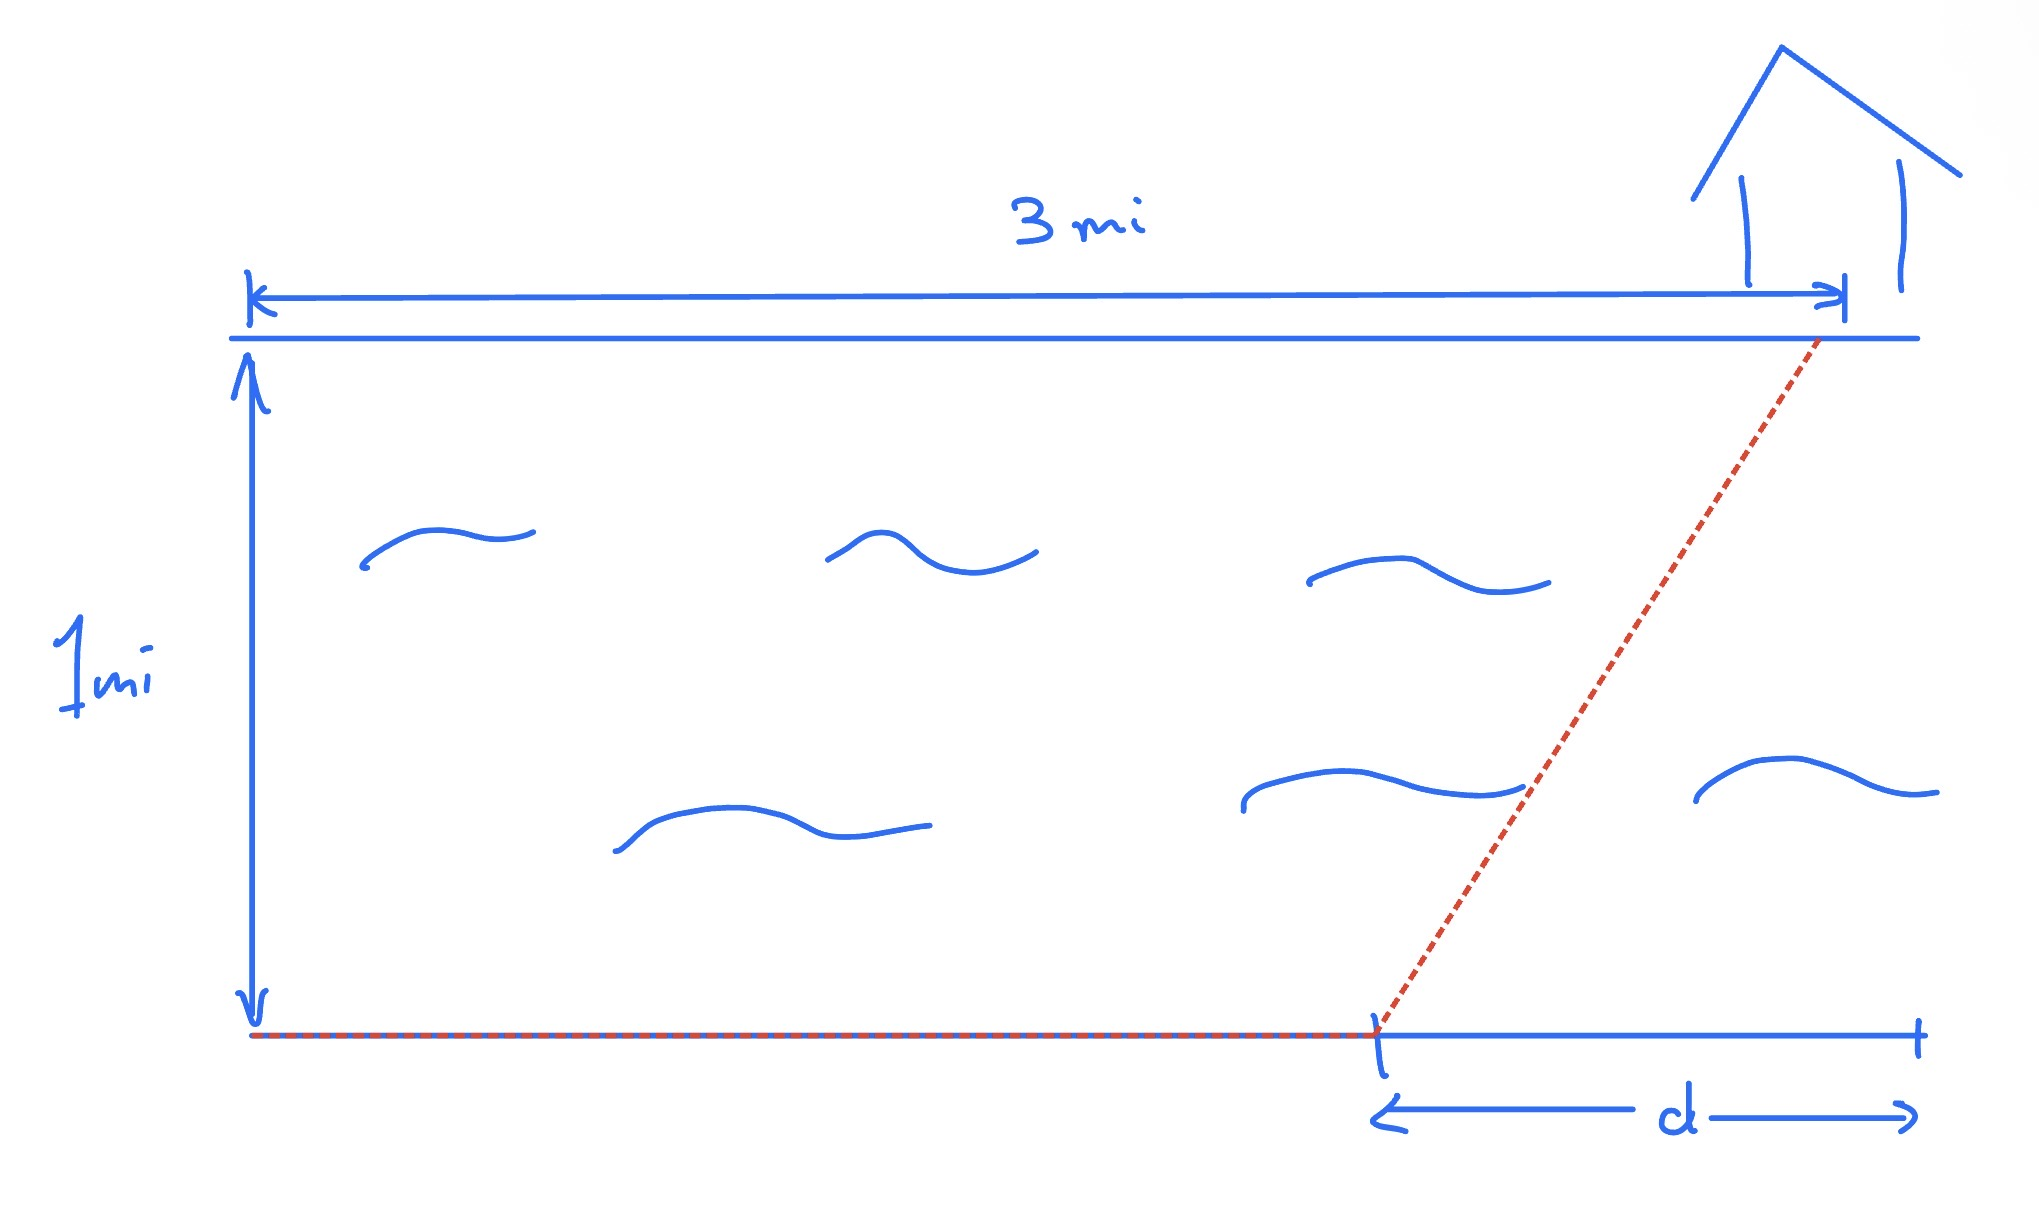
\includegraphics[width=0.8\textwidth]{IMG_2891.jpeg}
%\end{center}

\begin{enumerate}
\mpageT{.5}{.5}{
\item Suppose Bob wants to build a fence to enclose some sheep with a rectangular sheep pen. Fortunately, he lives next to a river, so he only needs to build three sides of the enclosure. Bob has $30$m of fencing. What are the dimensions that will enclose the greatest amount of sheep?
}{\graphicsC{sheepPen}{3}
}
{\bf Modeling Phase}
\tasksA{2}{
\task Create variables that describe the width and length of the sheep pen.
\task What quantity are we going to maximize? Let's call this quantity $S$.  Use both of your new variables to write down an equation for this quantity?\vs{1}
\task Bob's constraint is that he only has $30$m of fencing. Use your variables to write down an equation that represents this constraint.
\task Both the quantity you are going to maximize, $S$, and your constraint contain both of your variables. Use your constraint to solve for one variable and substitute  into $S$.
}
\vs{1}
{\bf Calculus Phase} Think about the process you have been using to optimize other quantities. Use that process here to find the dimension that maximize the area of the sheep pen?


\newpage
\item Suppose John is standing next to a river that is 1 mile wide. His house is on the opposite of the river 3 miles down. John can swim at 5 miles per hour but he can run at 8 miles per hour. What is the shortest amount of time it can take John to reach his house? You will find this by finding the best choice for $d$ where John stops running and starts swimming.\\
\mpageT{.4}{.6}[\hs{.1}]{
{\bf Modeling Phase} We first need to develop a model of the total time: $$T_{total}=T_{run}+T_{swim}$$
The total horizontal distance to the house is $3$ miles.  Once John starts to swim, the remaining horizontal distance is $d$ miles (see Figure 1). 
}{\graphicsC{runSwim}{4}{Figure 1}
}
\tasksA{2}{
\task What is the distance John ran? Your answer should contain $d$.
\task How long does it take for John to run this distance? This is $T_{run}$.  Your answer should contain $d$.\vs{.5}
\task What is the distance John swam?  {\em Hint}: You will want to utilize Pythagorean's Theorem to find this distance. Your answer should contain $d$.
\task How long does it take for John to swim this distance? This is $T_{swim}$.  Your answer should contain $d$. \vs{.75}
\task* What is $T_{total}$? Your answer will contain $d$\vs{.25}
}
{\bf Calculus Phase} Think about the process you have been using to optimize quantities. Use that process to find the minimum time it takes for John to get home. You will definitely want to use technology for the last part of finding critical numbers.


    \vfill













\end{enumerate}

\end{document}